\documentclass{article}
\usepackage{amsmath}
\usepackage{amssymb}
\usepackage{graphicx}
\usepackage{tikz}
\usepackage{pgfplots}
\pgfplotsset{compat=1.18}
\usepackage{booktabs}
\usepackage{xcolor}

\newenvironment{lesson-meta}{}{}
\newenvironment{item-analysis}{}{}
\newenvironment{model-discuss}{}{}
\newenvironment{concept-box}{}{}
\newenvironment{concept-summary}{}{}
\newenvironment{example}[1]{}{}
\newenvironment{tryit}[1]{}{}
\newenvironment{practice}[2]{}{}
\newenvironment{te-addendum}[2]{}{}
\newcommand{\answer}[1]{}
\newcommand{\placeholder}[2]{}
\newcommand{\uncertain}[2]{#1}
\newcommand{\te}[1]{}

\begin{document}

\begin{lesson-meta}
\textbf{5-1 $n$th Roots, Radicals, and Rational Exponents}

\textbf{I CAN...} relate roots and rational exponents and use them to simplify expressions and solve equations.

\textbf{VOCABULARY}
\begin{itemize}
    \item $n$th root
\end{itemize}

\textbf{ESSENTIAL QUESTION} How are exponents and radicals used to represent roots of real numbers?
\end{lesson-meta}

\begin{model-discuss}
\textbf{EXPLORE \& REASON}

The graph shows $y = x^2$.

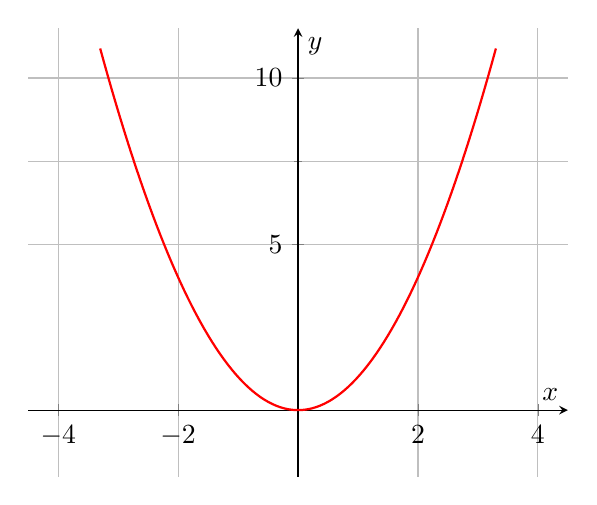
\begin{tikzpicture}
\begin{axis}[
    axis lines=center,
    xmin=-4.5, xmax=4.5,
    ymin=-2, ymax=11.5,
    xtick={-4, -2, 2, 4},
    ytick={5, 10},
    xlabel={$x$},
    ylabel={$y$},
    grid=both,
    minor tick num=1
]
\addplot[domain=-3.3:3.3, color=red, thick, samples=100] {x^2};
\end{axis}
\end{tikzpicture}

\textbf{A.} Find \textit{all} possible values of $x$ or $y$ so that the point is on the graph.
\begin{enumerate}
    \item[(a)] $(2, \rule{1cm}{0.15mm})$
    \item[(b)] $(3, \rule{1cm}{0.15mm})$
    \item[(c)] $(-3, \rule{1cm}{0.15mm})$
    \item[(d)] $(5, \rule{1cm}{0.15mm})$
    \item[(e)] $(\rule{1cm}{0.15mm}, 4)$
    \item[(f)] $(\rule{1cm}{0.15mm}, -16)$
    \item[(g)] $(\rule{1cm}{0.15mm}, 7)$
    \item[(h)] $(\rule{1cm}{0.15mm}, 5)$
\end{enumerate}

\textbf{B. Communicate Precisely} Write a precise set of instructions that show how to find an approximate value of $\sqrt{13}$ using the graph.

\textbf{C.} Draw a graph of $y = x^3$. Use the graph to approximate each value.
\begin{enumerate}
    \item[(a)] $\sqrt[3]{5}$
    \item[(b)] $\sqrt[3]{-5}$
    \item[(c)] $\sqrt[3]{8}$
    \item[(d)] A solution to $x^3 = 5$
    \item[(e)] A solution to $x^3 = -5$
    \item[(f)] A solution to $x^3 = 8$
\end{enumerate}
\end{model-discuss}

\textbf{MAKE SENSE AND PERSEVERE}
Recall that third degree polynomial functions have three solutions. Here, one solution is real and the other two are complex. How could you find the complex solutions?

\begin{example}{1}
\textbf{Find all Real $n$th Roots}

\textbf{A. What are all the real cube roots of 125?}

An \textbf{$n$th root} of a number $c$ is $x$, such that $x^n = c$. An $n$th root can be represented using a radical symbol by $x = \sqrt[n]{c}$.

Since $125 = 5^3$, $\sqrt[3]{125} = 5$ is a real cube root.

To determine if there are other real cube roots of 125, consider the function $f(x) = x^3 - 125$. The zeros of $f$ are the cube roots of 125.

The graph of $f$ has only one $x$-intercept. Therefore, 5 is the only real cube root of 125.

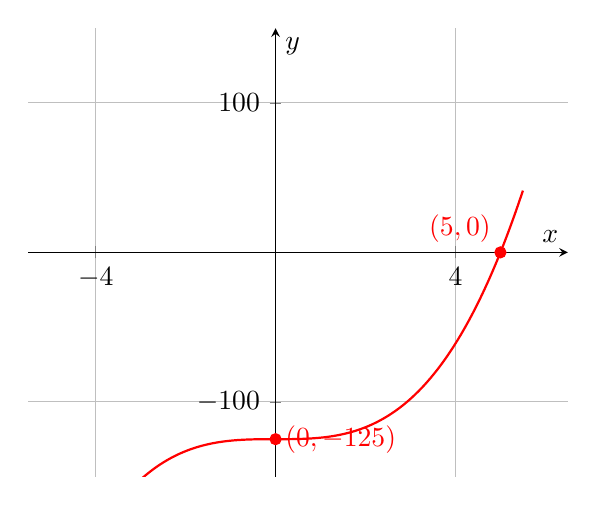
\begin{tikzpicture}
\begin{axis}[
    axis lines=center,
    xmin=-5.5, xmax=6.5,
    ymin=-150, ymax=150,
    xtick={-4, 4},
    ytick={-100, 100},
    xlabel={$x$},
    ylabel={$y$},
    grid=both
]
\addplot[domain=-3:5.5, color=red, thick, samples=100] {x^3 - 125};
\addplot[mark=*, color=red] coordinates {(5,0)} node[above left] {$(5,0)$};
\addplot[mark=*, color=red] coordinates {(0,-125)} node[right] {$(0,-125)$};
\end{axis}
\end{tikzpicture}

\textbf{B. What are all the real fourth roots of 16?}

\textbf{CONSTRUCT ARGUMENTS}
Consider the function $f(x) = x^4 - 16$. How can you use the graph of $f$ to conclude that 16 has two real fourth roots? \textbf{MP.3}

Since $16 = 2^4$, one fourth root is the principal root, $\sqrt[4]{16} = 2$.

To determine all the real fourth roots of 16, solve $x^4 = 16$.
\begin{align*}
x^4 &= 16 \\
x^4 - 16 &= 0 \\
(x^2 - 4)(x^2 + 4) &= 0 \\
(x - 2)(x + 2)(x^2 + 4) &= 0
\end{align*}
The zeros of the first two factors are 2 and $-2$. The zeros of the quadratic factor $x^2 + 4$ are imaginary. Therefore, the real fourth roots of 16 are 2 and $-2$.
\end{example}

\begin{tryit}{1}
Find the specified roots of each number.

\textbf{a.} real fourth roots of 81 \qquad \textbf{b.} real cube roots of 64
\end{tryit}

\textbf{CONCEPTUAL UNDERSTANDING}

\textbf{STUDY TIP}
It is important to recognize multiple representations of the same value so you can select the form that is most efficient for a given situation.

\begin{example}{2}
\textbf{Understand Rational Exponents}

\textbf{A. What is the meaning of the exponent in the expression $16^{\frac{1}{4}}$?}

Extend the properties of \textit{integer} exponents to \textit{rational} exponents.
\begin{align*}
16^{\frac{1}{4}} &= (2^4)^{\frac{1}{4}} \quad \text{Use the Power of a Power Property.} \\
&= 2^1 \\
&= \sqrt[4]{16} \quad \text{Since } 2 = \sqrt[4]{16}, 16 = 2^4.
\end{align*}
Therefore, $16^{\frac{1}{4}}$ is another way to represent $\sqrt[4]{16}$, or 2.

In general, for positive integer $n$, $x^{\frac{1}{n}}$ can be expressed as the radical $\sqrt[n]{x}$.
\[ x^{\frac{1}{n}} = \sqrt[n]{x} \]
Both the exponent $\frac{1}{n}$ and the radical symbol $\sqrt[n]{x}$ indicate the principal $n$th root.

\textbf{B. Write $27^{\frac{2}{3}}$ as a radical.}
\begin{align*}
27^{\frac{2}{3}} &= (27^{\frac{1}{3}})^2 \quad \text{Use the Power of a Power Property.} \\
&= (\sqrt[3]{27})^2 \\
&= 3^2 \\
&= 9
\end{align*}
This means that you can rewrite $27^{\frac{2}{3}}$ as $(\sqrt[3]{27})^2$. Since 27 is a perfect cube, you can evaluate the radical expression mentally by taking the cube root first and then squaring.
\[ 27^{\frac{2}{3}} = (\sqrt[3]{27})^2 = 3^2 = 9 \]
\end{example}

\begin{tryit}{2}
Explain what each fractional exponent means, then evaluate.

\textbf{a.} $25^{\frac{1}{2}}$ \qquad \textbf{b.} $32^{\frac{2}{5}}$
\end{tryit}

\begin{concept-box}
\textbf{CONCEPT Interpreting Rational Exponents}

In general, if the $n$th root of $c$ is a real number, $\sqrt[n]{c} = c^{\frac{1}{n}}$.

Furthermore, if $m$ is an integer, then
\[ c^{\frac{m}{n}} = (c^{\frac{1}{n}})^m = (\sqrt[n]{c})^m \quad \text{and} \quad \sqrt[n]{c^m} = (c^m)^{\frac{1}{n}} = c^{\frac{m}{n}}. \]
\end{concept-box}

\textbf{APPLICATION}

\textbf{USE APPROPRIATE TOOLS}
Many expressions with integer roots can be evaluated using mental math. However, when the root is not an integer, it is helpful to use the power function of a calculator to compute rational roots. \textbf{MP.5}

\begin{example}{3}
\textbf{Evaluate Expressions With Rational Exponents}

\textbf{A. Evaluate the expressions $32^{\frac{3}{5}}$, $27^{-\frac{2}{3}}$, and $50^{\frac{3}{4}}$.}

\begin{align*}
32^{\frac{3}{5}} &= (32^{\frac{1}{5}})^3 \\
&= 2^3 \\
&= 8
\end{align*}

\begin{align*}
27^{-\frac{2}{3}} &= (27^{\frac{1}{3}})^{-2} \\
&= (3)^{-2} \\
&= \frac{1}{9}
\end{align*}

Since 50 does not have a perfect 4th root, use a calculator to approximate:
\[ 50^{\frac{3}{4}} \approx 18.80 \]

\textbf{B. The Fujita scale rating, $F$, of a tornado is represented by $F = \sqrt[3]{\left(\frac{W}{14.1}\right)^2} - 2$, where $W$ is the estimated wind speed of the tornado in miles per hour. What is the Fujita scale rating for this tornado?}

\placeholder{photo}{A tornado on a road, with label 'Wind speed estimated at 100 mph'}

\begin{align*}
F &= \sqrt[3]{\left(\frac{100}{14.1}\right)^2} - 2 \\
&= \left(\frac{100}{14.1}\right)^{\frac{2}{3}} - 2 \\
&\approx (7.09)^{\frac{2}{3}} - 2 \\
&\approx 3.69 - 2 \\
&\approx 1.69
\end{align*}

A tornado with estimated wind speeds of 100 mph is classified as F1 according to the Fujita scale.
\end{example}

\begin{tryit}{3}
What is the value of each expression? Round to the nearest hundredth if necessary.

\textbf{a.} $-(16^{\frac{3}{4}})$ \qquad \textbf{b.} $\sqrt[5]{3.5^4}$
\end{tryit}

\begin{example}{4}
\textbf{Simplify $n$th Roots}

Simplify each expression. Assume all variables are positive.

\textbf{USE STRUCTURE}
You can also work this problem using the method in Part A. The exponents 20 and 8 are both multiples of 4. So you can rewrite this expression as $\sqrt[4]{x^{20}y^8} = \sqrt[4]{(x^5y^2)^4}$ which equals $x^5y^2$.

\textbf{A.} $\sqrt[5]{32m^{15}}$
\begin{align*}
\sqrt[5]{2^5m^{15}} &= \sqrt[5]{(2m^3)^5} \quad \text{Write the radicand as an expression to the 5th power.} \\
&= 2m^3
\end{align*}
So, $\sqrt[5]{32m^{15}} = 2m^3$.

\textbf{B.} $\sqrt[4]{x^{20}y^8}$
\begin{align*}
\sqrt[4]{x^{20}y^8} &= (x^{20}y^8)^{\frac{1}{4}} \quad \text{Raise the radicand to the one-fourth power.} \\
&= x^{\frac{20}{4}}y^{\frac{8}{4}} \\
&= x^5y^2
\end{align*}
So, $\sqrt[4]{x^{20}y^8} = x^5y^2$.
\end{example}

\begin{tryit}{4}
Simplify each expression.

\textbf{a.} $\sqrt[3]{-8a^3b^9}$ \qquad \textbf{b.} $\sqrt[4]{256x^{12}y^{24}}$
\end{tryit}

\textbf{GENERALIZE}
Raise both sides of the equation to a power so that the exponent of the variable becomes 1. Using the Power of a Power Property, $(x^n)^{\frac{1}{n}} = x^1$.

\begin{example}{5}
\textbf{Use $n$th Roots to Solve Equations}

\textbf{Solve the equation $2x^5 = 64$.}

\textbf{A.} $2x^5 = 64$
\begin{align*}
x^5 &= 32 \\
(x^5)^{\frac{1}{5}} &= 32^{\frac{1}{5}} \quad \text{Raise each side of the equation to the } \frac{1}{5} \text{ power.} \\
x &= 2
\end{align*}

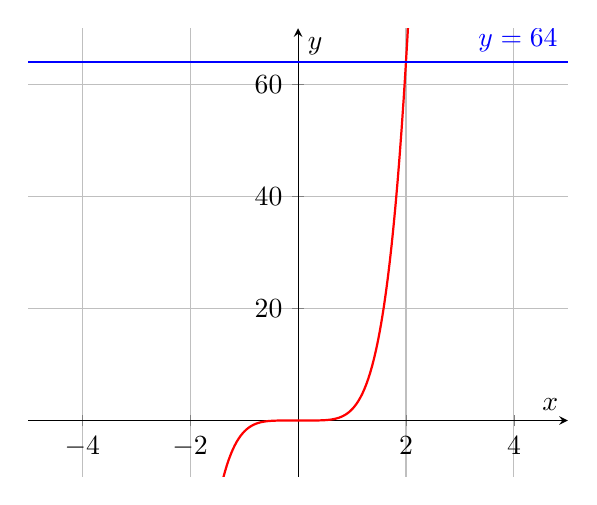
\begin{tikzpicture}
\begin{axis}[
    axis lines=center,
    xmin=-5, xmax=5,
    ymin=-10, ymax=70,
    xtick={-4, -2, 2, 4},
    ytick={20, 40, 60},
    xlabel={$x$},
    ylabel={$y$},
    grid=both
]
\addplot[domain=-1.5:2.1, color=red, thick, samples=100] {2*x^5} node[right] {$y = 2x^5$};
\addplot[domain=-5:5, color=blue, thick] {64} node[above left] {$y = 64$};
\end{axis}
\end{tikzpicture}

The graph shows one point of intersection, so there is only one real solution.
The solution to the equation is $x = 2$.

\textbf{B.} $3x^4 = 1875$
\begin{align*}
x^4 &= 625 \\
(x^4)^{\frac{1}{4}} &= \pm(625)^{\frac{1}{4}} \quad \text{A negative integer raised to an even power is positive, so $-5$ is also a real solution.} \\
x &= \pm 5
\end{align*}

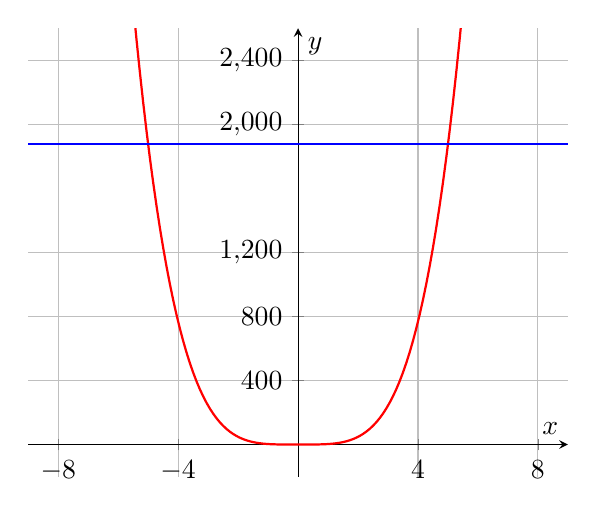
\begin{tikzpicture}
\begin{axis}[
    axis lines=center,
    xmin=-9, xmax=9,
    ymin=-200, ymax=2600,
    xtick={-8, -4, 4, 8},
    ytick={400, 800, 1200, 2000, 2400},
    xlabel={$x$},
    ylabel={$y$},
    grid=both
]
\addplot[domain=-5.5:5.5, color=red, thick, samples=100] {3*x^4} node[left] {$y = 3x^4$};
\addplot[domain=-9:9, color=blue, thick] {1875} node[below right] {$y = 1875$};
\end{axis}
\end{tikzpicture}

The graphs show 2 points of intersection, so there are no other real solutions.
The solutions are $x = \pm 5$.
\end{example}

\begin{tryit}{5}
\textbf{a.} Solve the equation $5x^3 = 320$.

\textbf{b.} Solve the equation $2p^4 = 162$.
\end{tryit}

\begin{concept-box}
\textbf{CONCEPT Solving an Equation in the Form $x^n = c$}

To solve an equation in the form $x^n = c$, find the $n$th root of both sides by raising each expression to the $\frac{1}{n}$ power.
\[ (x^n)^{\frac{1}{n}} = (c)^{\frac{1}{n}} \]
\end{concept-box}

\textbf{APPLICATION}

\textbf{MODEL WITH MATHEMATICS}
Use the information in the problem to write an equation that models the situation. \textbf{MP.4}

\begin{example}{6}
\textbf{Use $n$th Roots to Solve Problems}

A garden water fountain is made of two cubes. The larger container has an edge length 2 cm longer than the edge length of a second cube. When the larger cube empties into the smaller cube, how much water will spill over the edge of the smaller cube into the base?

\placeholder{illustration}{A garden water fountain made of a smaller cube sitting on a larger cube. Water flows into the smaller cube and spills over into the larger one. Label 'The volume of the larger cube is 729 cm$^3$'.}

\begin{align*}
(x + 2)^3 &= 729 \\
[(x + 2)^3]^{\frac{1}{3}} &= (729)^{\frac{1}{3}} \quad \text{Raise both sides to the } \frac{1}{3} \text{ power and solve.} \\
x + 2 &= 9 \\
x &= 7
\end{align*}

The volume of the smaller cube is $7^3$, or $343 \text{ cm}^3$.

The volume of the larger cube is $729 \text{ cm}^3$.

The amount of water that spills is $729 - 343 = 386$.

When the larger cube empties into the smaller cube, $386 \text{ cm}^3$ of water will spill out into the base of the fountain.
\end{example}

\begin{tryit}{6}
One cube has an edge length $3 \text{ cm}$ shorter than the edge length of a second cube. The volume of the smaller cube is $200 \text{ cm}^3$. What is the volume of the larger cube?
\end{tryit}

\begin{concept-summary}
\textbf{CONCEPT SUMMARY $n$th Roots, Radicals, and Rational Exponents}

\textbf{WORDS}
\begin{itemize}
    \item \textbf{Relating Radical and Exponential Forms}
    The index of a radical is equivalent to the denominator of a fractional exponent. The exponent of the radicand is equivalent to the numerator of a fractional exponent.
    \item \textbf{Solving an Equation in the Form $x^n = c$}
    To solve an equation in the form $x^n = c$, find the $n$th root of both sides of the equation by raising each expression to the $\frac{1}{n}$ power.
\end{itemize}

\textbf{NUMBERS}
\begin{itemize}
    \item Radical Form: $\sqrt[5]{32^4} = (32^4)^{\frac{1}{5}} = 32^{\frac{4}{5}}$
    \item Exponential Form: $729^{\frac{5}{6}} = (729^{\frac{1}{6}})^5 = (\sqrt[6]{729})^5$
    \item $x^3 = 1,728 \rightarrow (x^3)^{\frac{1}{3}} = (1,728)^{\frac{1}{3}} \rightarrow x = 12$
\end{itemize}

\textbf{ALGEBRA}
\begin{itemize}
    \item Radical Form: $\sqrt[n]{c^m} = (c^m)^{\frac{1}{n}} = c^{\frac{m}{n}}$
    \item Exponential Form: $c^{\frac{m}{n}} = (c^{\frac{1}{n}})^m = (\sqrt[n]{c})^m$
    \item $x^n = c \rightarrow (x^n)^{\frac{1}{n}} = (c)^{\frac{1}{n}} \rightarrow x = c^{\frac{1}{n}}$
\end{itemize}
\end{concept-summary}

\textbf{Do You UNDERSTAND?}

\begin{practice}{1}{}
\textbf{ESSENTIAL QUESTION} How are exponents and radicals used to represent roots of real numbers?
\end{practice}

\begin{practice}{2}{}
\textbf{Error Analysis} Kaitlyn said $\sqrt[3]{10} = 10^3$. Explain Kaitlyn's error.
\end{practice}

\begin{practice}{3}{}
\textbf{Vocabulary} In the radical expression $\sqrt[5]{125}$, what is the index? What is the radicand?
\end{practice}

\begin{practice}{4}{}
\textbf{Use Structure} Why is $75^{\frac{3}{5}}$ equal to $(75^{\frac{1}{5}})^3$?
\end{practice}

\begin{practice}{5}{}
\textbf{Construct Arguments} Amani said that $(x^8)^{\frac{1}{4}} = \frac{x^8}{x^4} = x^4$. Is Amani correct? Explain.
\end{practice}

\begin{practice}{6}{}
\textbf{Make Sense and Persevere} Is it possible for a rational exponent to be an improper fraction? Explain how $27^{\frac{4}{3}}$ is evaluated or why it cannot be evaluated.
\end{practice}

\textbf{Do You KNOW HOW?}

Write each expression in radical form.
\begin{practice}{7}{}
$a^{\frac{1}{5}}$
\end{practice}
\begin{practice}{8}{}
$7^{\frac{2}{3}}$
\end{practice}

Write each expression in exponential form.
\begin{practice}{9}{}
$\sqrt[3]{b}$
\end{practice}
\begin{practice}{10}{}
$\sqrt[4]{p^7}$
\end{practice}

\begin{practice}{11}{}
How many real third roots does $1,728$ have?
\end{practice}

\begin{practice}{12}{}
How many real sixth roots does $15,625$ have?
\end{practice}

\begin{practice}{13}{}
Solve the equation $4x^3 = 324$.
\end{practice}

\begin{practice}{14}{}
Solve the equation $2x^4 = 2,500$.
\end{practice}

Simplify each expression. Assume all variables are positive.
\begin{practice}{15}{}
$\sqrt[3]{27x^{12}y^6}$
\end{practice}
\begin{practice}{16}{}
$\sqrt[5]{-32x^5y^{30}}$
\end{practice}

\begin{practice}{17}{}
A snow globe is packaged in a cubic container that has volume $64 \text{ in.}^3$. A large shipping container is also a cube, and its edge length is $8 \text{ inches}$ longer than the edge length of the snow globe container. How many snow globes can fit into the larger shipping container?
\end{practice}

\textbf{PRACTICE \& PROBLEM SOLVING}

\textbf{UNDERSTAND}

\begin{practice}{18}{}
\textbf{Construct Arguments} Justice found that the fifth root of $243x^{15}y^5$ is $3x^3y$. Is Justice correct? Explain your reasoning. \textbf{MP.3}
\end{practice}

\begin{practice}{19}{}
\textbf{Make Sense and Persevere} For a show, spheres were bounced and passed. Explain how to find the radius $r$ of one of the inflated spheres. Use technology to compute your answer. \textbf{MP.1}

\placeholder{photo}{Many large colorful inflated spheres floating above a crowd. Label 'Volume of a sphere is $4,186 \frac{2}{3} \text{ in.}^3$'.}
\end{practice}

\begin{practice}{20}{}
\textbf{Error Analysis} Describe and correct the error a student made in writing this exponential expression in radical form. \textbf{MP.3}

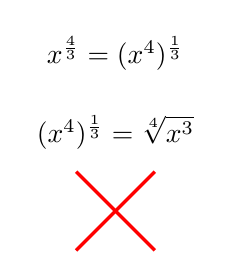
\begin{tikzpicture}
\node at (0, 0) {$x^{\frac{4}{3}} = (x^4)^{\frac{1}{3}}$};
\node at (0, -1) {$(x^4)^{\frac{1}{3}} = \sqrt[4]{x^3}$};
\draw[red, very thick] (-0.5, -1.5) -- (0.5, -2.5);
\draw[red, very thick] (-0.5, -2.5) -- (0.5, -1.5);
\end{tikzpicture}
\end{practice}

\begin{practice}{21}{}
\textbf{Construct Arguments} Determine whether $\sqrt[3]{x^2}$ is equal to $(\sqrt[3]{x})^2$. Explain your reasoning. \textbf{MP.3}
\end{practice}

\begin{practice}{22}{}
\textbf{Use Structure} How many third roots does $-512$ have? Explain your reasoning. \textbf{MP.7}
\end{practice}

\begin{practice}{23}{}
\textbf{Higher Order Thinking} The annual interest formula below calculates the final balance of an account, $F$, given a starting balance, $S$, and an interest rate, $r$, after 10 years.
\[ F = S(1 + r)^{10} \]
When solving for $r$, why can the negative root be ignored?
\end{practice}

\begin{practice}{24}{}
\textbf{Mathematical Connections} The lengths of the two legs of a right triangle are $4$ and $8$. What is the length of the hypotenuse, in simplest radical form?
\end{practice}

\textbf{PRACTICE}

Find the specified roots of each number. SEE EXAMPLE 1
\begin{practice}{25}{}
the real fourth roots of $81$
\end{practice}
\begin{practice}{26}{}
the real third roots of $343$
\end{practice}
\begin{practice}{27}{}
the real fifth roots of $1,024$
\end{practice}
\begin{practice}{28}{}
the real square roots of $25$
\end{practice}

Rewrite each expression using a fractional exponent. SEE EXAMPLE 2
\begin{practice}{29}{}
$\sqrt[6]{16^2}$
\end{practice}
\begin{practice}{30}{}
$\sqrt[6]{729}$
\end{practice}
\begin{practice}{31}{}
$\sqrt[3]{x^2}$
\end{practice}
\begin{practice}{32}{}
$\sqrt[4]{ab}$
\end{practice}

What is the value of each expression? Round to the nearest hundredth if necessary. SEE EXAMPLE 3
\begin{practice}{33}{}
$\sqrt[4]{25^2}$
\end{practice}
\begin{practice}{34}{}
$-\sqrt[3]{125^5}$
\end{practice}

Simplify each expression. Assume all variables are positive. SEE EXAMPLE 4
\begin{practice}{35}{}
$\sqrt[3]{8y^9}$
\end{practice}
\begin{practice}{36}{}
$\sqrt[4]{q^{12}z^4}$
\end{practice}
\begin{practice}{37}{}
$\sqrt[6]{729a^{24}b^{18}}$
\end{practice}
\begin{practice}{38}{}
$\sqrt[8]{v^8g^{40}}$
\end{practice}

Solve each equation. SEE EXAMPLE 5
\begin{practice}{39}{}
$1,125 = 9x^3$
\end{practice}
\begin{practice}{40}{}
$6,480 = 5w^4$
\end{practice}
\begin{practice}{41}{}
$270 = 10q^3$
\end{practice}
\begin{practice}{42}{}
$256 = 4h^6$
\end{practice}

\begin{practice}{43}{}
A small cube holds chocolate candies. Its side length is $1.5 \text{ in.}$ smaller than a second, larger cube of chocolate candies. What is the volume of the larger cube? SEE EXAMPLE 6

\placeholder{illustration}{Two cubes of chocolate. Smaller cube labeled 'Volume is 85 in.$^3$' with 'DARK Chocolate' on it. Larger cube with 'Milk CHOCOLATE' on it.}
\end{practice}

\textbf{APPLY}

\begin{practice}{44}{}
\textbf{Model With Mathematics} A water-walking ball has a set volume. What is the radius, $r$, of the ball?

\placeholder{illustration}{Person inside a transparent inflatable ball walking on water. Label 'volume $\approx 4.19 \text{ m}^3$'.}
\end{practice}

\begin{practice}{45}{}
\textbf{Make Sense and Persevere} Ahmed received a box of gifts. The box is a rectangular prism with the same height and width, and the length is twice the width. The volume of the box is $3,456 \text{ in.}^3$. What is the height of the box?

\placeholder{illustration}{A rectangular prism box labeled 'Mystery BOX' with gifts flowing out. Dimensions marked: depth is $x \text{ in.}$, height is $x \text{ in.}$, width is $2x \text{ in.}$}
\end{practice}

\begin{practice}{46}{}
\textbf{Make Sense and Persevere} Amelia's bank account earns interest annually. The equation shows her starting balance of $\$200$ and her balance at the end of four years, $\$220.82$. At what rate, $r$, did Amelia earn interest?
\[ 220.82 = 200(1 + r)^4 \]
\end{practice}

\begin{practice}{47}{}
\textbf{Model With Mathematics} One measure of a patient's body surface area is found using the expression $\sqrt{\frac{H \cdot W}{3,600}}$. Write this with a fractional exponent.
\end{practice}

\textbf{ASSESSMENT PRACTICE}

\begin{practice}{48}{}
Determine if each expression is another way to write $b^{\frac{3}{4}}$. Select \textit{Yes} or \textit{No}.

\begin{tabular}{lcc}
\toprule
& \textbf{Yes} & \textbf{No} \\
\midrule
a. $\sqrt[4]{b^3}$ & $\square$ & $\square$ \\
b. $(b^3)^{\frac{1}{4}}$ & $\square$ & $\square$ \\
c. $b^{\frac{4}{3}}$ & $\square$ & $\square$ \\
d. $\sqrt[3]{b^4}$ & $\square$ & $\square$ \\
e. $\frac{b^3}{b^4}$ & $\square$ & $\square$ \\
\bottomrule
\end{tabular}
\end{practice}

\begin{practice}{49}{}
\textbf{SAT/ACT} Which of the following is equivalent to $\sqrt[6]{4,096x^{18}y^{30}}$, where $x > 0$ and $y > 0$?
\begin{enumerate}
    \item[A] $682.7x^{15}y^{24}$
    \item[B] $4x^{1.6}y^{1.8}$
    \item[C] $4,096x^3y^5$
    \item[D] $4x^3y^5$
    \item[E] $682.7x^3y^5$
\end{enumerate}
\end{practice}

\begin{practice}{50}{}
\textbf{Performance Task} A milk processing company uses cylindrical-shaped containers. The height of the container is equal to the diameter of the base.

\placeholder{illustration}{A cylindrical milk container inside a processing facility. Label 'volume $169.65 \text{ ft}^3$'.}

\textbf{Part A} How much material is needed to make the lateral surface area of the shipping container?

\textbf{Part B} The cargo hold of a ship is $20 \text{ ft}$ high. What is the largest number of these shipping containers that could be stacked on top of each other inside the cargo hold?
\end{practice}

\end{document}